\documentclass[1p]{elsarticle_modified}
%\bibliographystyle{elsarticle-num}

%\usepackage[colorlinks]{hyperref}
%\usepackage{abbrmath_seonhwa} %\Abb, \Ascr, \Acal ,\Abf, \Afrak
\usepackage{amsfonts}
\usepackage{amssymb}
\usepackage{amsmath}
\usepackage{amsthm}
\usepackage{scalefnt}
\usepackage{amsbsy}
\usepackage{kotex}
\usepackage{caption}
\usepackage{subfig}
\usepackage{color}
\usepackage{graphicx}
\usepackage{xcolor} %% white, black, red, green, blue, cyan, magenta, yellow
\usepackage{float}
\usepackage{setspace}
\usepackage{hyperref}

\usepackage{tikz}
\usetikzlibrary{arrows}

\usepackage{multirow}
\usepackage{array} % fixed length table
\usepackage{hhline}

%%%%%%%%%%%%%%%%%%%%%
\makeatletter
\renewcommand*\env@matrix[1][\arraystretch]{%
	\edef\arraystretch{#1}%
	\hskip -\arraycolsep
	\let\@ifnextchar\new@ifnextchar
	\array{*\c@MaxMatrixCols c}}
\makeatother %https://tex.stackexchange.com/questions/14071/how-can-i-increase-the-line-spacing-in-a-matrix
%%%%%%%%%%%%%%%

\usepackage[normalem]{ulem}

\newcommand{\msout}[1]{\ifmmode\text{\sout{\ensuremath{#1}}}\else\sout{#1}\fi}
%SOURCE: \msout is \stkout macro in https://tex.stackexchange.com/questions/20609/strikeout-in-math-mode

\newcommand{\cancel}[1]{
	\ifmmode
	{\color{red}\msout{#1}}
	\else
	{\color{red}\sout{#1}}
	\fi
}

\newcommand{\add}[1]{
	{\color{blue}\uwave{#1}}
}

\newcommand{\replace}[2]{
	\ifmmode
	{\color{red}\msout{#1}}{\color{blue}\uwave{#2}}
	\else
	{\color{red}\sout{#1}}{\color{blue}\uwave{#2}}
	\fi
}

\newcommand{\Sol}{\mathcal{S}} %segment
\newcommand{\D}{D} %diagram
\newcommand{\A}{\mathcal{A}} %arc


%%%%%%%%%%%%%%%%%%%%%%%%%%%%%5 test

\def\sl{\operatorname{\textup{SL}}(2,\Cbb)}
\def\psl{\operatorname{\textup{PSL}}(2,\Cbb)}
\def\quan{\mkern 1mu \triangleright \mkern 1mu}

\theoremstyle{definition}
\newtheorem{thm}{Theorem}[section]
\newtheorem{prop}[thm]{Proposition}
\newtheorem{lem}[thm]{Lemma}
\newtheorem{ques}[thm]{Question}
\newtheorem{cor}[thm]{Corollary}
\newtheorem{defn}[thm]{Definition}
\newtheorem{exam}[thm]{Example}
\newtheorem{rmk}[thm]{Remark}
\newtheorem{alg}[thm]{Algorithm}

\newcommand{\I}{\sqrt{-1}}
\begin{document}

%\begin{frontmatter}
%
%\title{Boundary parabolic representations of knots up to 8 crossings}
%
%%% Group authors per affiliation:
%\author{Yunhi Cho} 
%\address{Department of Mathematics, University of Seoul, Seoul, Korea}
%\ead{yhcho@uos.ac.kr}
%
%
%\author{Seonhwa Kim} %\fnref{s_kim}}
%\address{Center for Geometry and Physics, Institute for Basic Science, Pohang, 37673, Korea}
%\ead{ryeona17@ibs.re.kr}
%
%\author{Hyuk Kim}
%\address{Department of Mathematical Sciences, Seoul National University, Seoul 08826, Korea}
%\ead{hyukkim@snu.ac.kr}
%
%\author{Seokbeom Yoon}
%\address{Department of Mathematical Sciences, Seoul National University, Seoul, 08826,  Korea}
%\ead{sbyoon15@snu.ac.kr}
%
%\begin{abstract}
%We find all boundary parabolic representation of knots up to 8 crossings.
%
%\end{abstract}
%\begin{keyword}
%    \MSC[2010] 57M25 
%\end{keyword}
%
%\end{frontmatter}

%\linenumbers
%\tableofcontents
%
\newcommand\colored[1]{\textcolor{white}{\rule[-0.35ex]{0.8em}{1.4ex}}\kern-0.8em\color{red} #1}%
%\newcommand\colored[1]{\textcolor{white}{ #1}\kern-2.17ex	\textcolor{white}{ #1}\kern-1.81ex	\textcolor{white}{ #1}\kern-2.15ex\color{red}#1	}

{\Large $\underline{12n_{0387}~(K12n_{0387})}$}

\setlength{\tabcolsep}{10pt}
\renewcommand{\arraystretch}{1.6}
\vspace{1cm}\begin{tabular}{m{100pt}>{\centering\arraybackslash}m{274pt}}
\multirow{5}{120pt}{
	\centering
	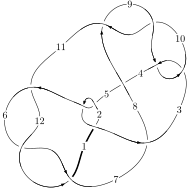
\includegraphics[width=112pt]{../../../GIT/diagram.site/Diagrams/png/2476_12n_0387.png}\\
\ \ \ A knot diagram\footnotemark}&
\allowdisplaybreaks
\textbf{Linearized knot diagam} \\
\cline{2-2}
 &
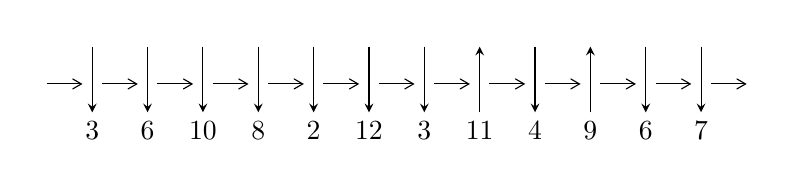
\begin{tikzpicture}[x=20pt, y=17pt]
	% nodes
	\node (C0) at (0, 0) {};
	\node (C1) at (1, 0) {};
	\node (C1U) at (1, +1) {};
	\node (C1D) at (1, -1) {3};

	\node (C2) at (2, 0) {};
	\node (C2U) at (2, +1) {};
	\node (C2D) at (2, -1) {6};

	\node (C3) at (3, 0) {};
	\node (C3U) at (3, +1) {};
	\node (C3D) at (3, -1) {10};

	\node (C4) at (4, 0) {};
	\node (C4U) at (4, +1) {};
	\node (C4D) at (4, -1) {8};

	\node (C5) at (5, 0) {};
	\node (C5U) at (5, +1) {};
	\node (C5D) at (5, -1) {2};

	\node (C6) at (6, 0) {};
	\node (C6U) at (6, +1) {};
	\node (C6D) at (6, -1) {12};

	\node (C7) at (7, 0) {};
	\node (C7U) at (7, +1) {};
	\node (C7D) at (7, -1) {3};

	\node (C8) at (8, 0) {};
	\node (C8U) at (8, +1) {};
	\node (C8D) at (8, -1) {11};

	\node (C9) at (9, 0) {};
	\node (C9U) at (9, +1) {};
	\node (C9D) at (9, -1) {4};

	\node (C10) at (10, 0) {};
	\node (C10U) at (10, +1) {};
	\node (C10D) at (10, -1) {9};

	\node (C11) at (11, 0) {};
	\node (C11U) at (11, +1) {};
	\node (C11D) at (11, -1) {6};

	\node (C12) at (12, 0) {};
	\node (C12U) at (12, +1) {};
	\node (C12D) at (12, -1) {7};
	\node (C13) at (13, 0) {};

	% arrows
	\draw[->,>={angle 60}]
	(C0) edge (C1) (C1) edge (C2) (C2) edge (C3) (C3) edge (C4) (C4) edge (C5) (C5) edge (C6) (C6) edge (C7) (C7) edge (C8) (C8) edge (C9) (C9) edge (C10) (C10) edge (C11) (C11) edge (C12) (C12) edge (C13) ;	\draw[->,>=stealth]
	(C1U) edge (C1D) (C2U) edge (C2D) (C3U) edge (C3D) (C4U) edge (C4D) (C5U) edge (C5D) (C6U) edge (C6D) (C7U) edge (C7D) (C8D) edge (C8U) (C9U) edge (C9D) (C10D) edge (C10U) (C11U) edge (C11D) (C12U) edge (C12D) ;
	\end{tikzpicture} \\
\hhline{~~} \\& 
\textbf{Solving Sequence} \\ \cline{2-2} 
 &
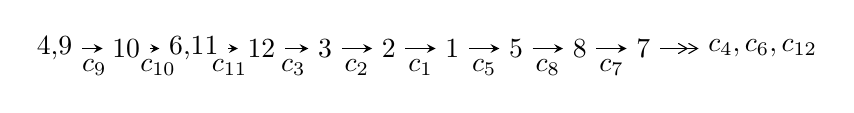
\begin{tikzpicture}[x=23pt, y=7pt]
	% node
	\node (A0) at (-1/8, 0) {4,9};
	\node (A1) at (1, 0) {10};
	\node (A2) at (33/16, 0) {6,11};
	\node (A3) at (25/8, 0) {12};
	\node (A4) at (33/8, 0) {3};
	\node (A5) at (41/8, 0) {2};
	\node (A6) at (49/8, 0) {1};
	\node (A7) at (57/8, 0) {5};
	\node (A8) at (65/8, 0) {8};
	\node (A9) at (73/8, 0) {7};
	\node (C1) at (1/2, -1) {$c_{9}$};
	\node (C2) at (3/2, -1) {$c_{10}$};
	\node (C3) at (21/8, -1) {$c_{11}$};
	\node (C4) at (29/8, -1) {$c_{3}$};
	\node (C5) at (37/8, -1) {$c_{2}$};
	\node (C6) at (45/8, -1) {$c_{1}$};
	\node (C7) at (53/8, -1) {$c_{5}$};
	\node (C8) at (61/8, -1) {$c_{8}$};
	\node (C9) at (69/8, -1) {$c_{7}$};
	\node (A10) at (11, 0) {$c_{4},c_{6},c_{12}$};

	% edge
	\draw[->,>=stealth]	
	(A0) edge (A1) (A1) edge (A2) (A2) edge (A3) (A3) edge (A4) (A4) edge (A5) (A5) edge (A6) (A6) edge (A7) (A7) edge (A8) (A8) edge (A9) ;
	\draw[->>,>={angle 60}]	
	(A9) edge (A10);
\end{tikzpicture} \\ 

\end{tabular} \\

\footnotetext{
The image of knot diagram is generated by the software ``\textbf{Draw programme}" developed by Andrew Bartholomew(\url{http://www.layer8.co.uk/maths/draw/index.htm\#Running-draw}), where we modified some parts for our purpose(\url{https://github.com/CATsTAILs/LinksPainter}).
}\phantom \\ \newline 
\centering \textbf{Ideals for irreducible components\footnotemark of $X_{\text{par}}$} 
 
\begin{align*}
I^u_{1}&=\langle 
-2 u^{14}+3 u^{13}-7 u^{12}+6 u^{11}-13 u^{10}+6 u^9-12 u^8-9 u^6-10 u^5+u^4-13 u^3+u^2+b-7 u-3,\\
\phantom{I^u_{1}}&\phantom{= \langle  }3 u^{15}-9 u^{14}+\cdots+2 a-8,\;u^{16}-3 u^{15}+\cdots+2 u+2\rangle \\
I^u_{2}&=\langle 
u^2+b+u+1,\;- u^3+2 a+u+2,\;u^4+u^2+2\rangle \\
I^u_{3}&=\langle 
- u^3+a u- u^2+b+1,\;- u^3 a-2 u^2 a+u^3+a^2-2 a u-2 u^2-1,\;u^4+u^3+u^2+1\rangle \\
I^u_{4}&=\langle 
- u^3- u^2+b+1,\;- u^3- u^2+a- u,\;u^4+1\rangle \\
I^u_{5}&=\langle 
b- u,\;a-1,\;u^2+1\rangle \\
\\
I^v_{1}&=\langle 
a,\;b+1,\;v+1\rangle \\
\end{align*}
\raggedright * 6 irreducible components of $\dim_{\mathbb{C}}=0$, with total 35 representations.\\
\footnotetext{All coefficients of polynomials are rational numbers. But the coefficients are sometimes approximated in decimal forms when there is not enough margin.}
\newpage
\renewcommand{\arraystretch}{1}
\centering \section*{I. $I^u_{1}= \langle -2 u^{14}+3 u^{13}+\cdots+b-3,\;3 u^{15}-9 u^{14}+\cdots+2 a-8,\;u^{16}-3 u^{15}+\cdots+2 u+2 \rangle$}
\flushleft \textbf{(i) Arc colorings}\\
\begin{tabular}{m{7pt} m{180pt} m{7pt} m{180pt} }
\flushright $a_{4}=$&$\begin{pmatrix}0\\u\end{pmatrix}$ \\
\flushright $a_{9}=$&$\begin{pmatrix}1\\0\end{pmatrix}$ \\
\flushright $a_{10}=$&$\begin{pmatrix}1\\u^2\end{pmatrix}$ \\
\flushright $a_{6}=$&$\begin{pmatrix}-\frac{3}{2} u^{15}+\frac{9}{2} u^{14}+\cdots+5 u+4\\2 u^{14}-3 u^{13}+\cdots+7 u+3\end{pmatrix}$ \\
\flushright $a_{11}=$&$\begin{pmatrix}u^2+1\\u^2\end{pmatrix}$ \\
\flushright $a_{12}=$&$\begin{pmatrix}-\frac{1}{2} u^{15}+\frac{1}{2} u^{14}+\cdots+\frac{3}{2} u^3+1\\- u^{15}+2 u^{14}+\cdots+u+1\end{pmatrix}$ \\
\flushright $a_{3}=$&$\begin{pmatrix}u\\u^3+u\end{pmatrix}$ \\
\flushright $a_{2}=$&$\begin{pmatrix}-\frac{1}{2} u^{15}+\frac{1}{2} u^{14}+\cdots- u^2+u\\- u^{15}+2 u^{14}+\cdots+2 u+1\end{pmatrix}$ \\
\flushright $a_{1}=$&$\begin{pmatrix}-\frac{3}{2} u^{15}+\frac{3}{2} u^{14}+\cdots+\frac{3}{2} u^3-3 u^2\\-4 u^{15}+9 u^{14}+\cdots+7 u+5\end{pmatrix}$ \\
\flushright $a_{5}=$&$\begin{pmatrix}- u^9-2 u^7-3 u^5-2 u^3- u\\- u^9- u^7- u^5+u\end{pmatrix}$ \\
\flushright $a_{8}=$&$\begin{pmatrix}u^4+u^2+1\\u^4\end{pmatrix}$ \\
\flushright $a_{7}=$&$\begin{pmatrix}- u^8- u^6- u^4+1\\- u^{10}-2 u^8-3 u^6-2 u^4- u^2\end{pmatrix}$\\&\end{tabular}
\flushleft \textbf{(ii) Obstruction class $= -1$}\\~\\
\flushleft \textbf{(iii) Cusp Shapes $= 2 u^{15}-8 u^{14}+12 u^{13}-18 u^{12}+18 u^{11}-28 u^{10}+12 u^9-16 u^8-2 u^7-8 u^6-30 u^5+10 u^4-20 u^3-4 u^2-10 u-20$}\\~\\
\newpage\renewcommand{\arraystretch}{1}
\flushleft \textbf{(iv) u-Polynomials at the component}\newline \\
\begin{tabular}{m{50pt}|m{274pt}}
Crossings & \hspace{64pt}u-Polynomials at each crossing \\
\hline $$\begin{aligned}c_{1}\end{aligned}$$&$\begin{aligned}
&u^{16}+31 u^{15}+\cdots+18 u+1
\end{aligned}$\\
\hline $$\begin{aligned}c_{2},c_{5},c_{6}\\c_{11},c_{12}\end{aligned}$$&$\begin{aligned}
&u^{16}+u^{15}+\cdots+9 u^2-1
\end{aligned}$\\
\hline $$\begin{aligned}c_{3},c_{9}\end{aligned}$$&$\begin{aligned}
&u^{16}-3 u^{15}+\cdots+2 u+2
\end{aligned}$\\
\hline $$\begin{aligned}c_{4}\end{aligned}$$&$\begin{aligned}
&u^{16}+15 u^{15}+\cdots+1866 u+314
\end{aligned}$\\
\hline $$\begin{aligned}c_{7}\end{aligned}$$&$\begin{aligned}
&u^{16}-3 u^{15}+\cdots+110 u+50
\end{aligned}$\\
\hline $$\begin{aligned}c_{8},c_{10}\end{aligned}$$&$\begin{aligned}
&u^{16}-5 u^{15}+\cdots+20 u+4
\end{aligned}$\\
\hline
\end{tabular}\\~\\
\newpage\renewcommand{\arraystretch}{1}
\flushleft \textbf{(v) Riley Polynomials at the component}\newline \\
\begin{tabular}{m{50pt}|m{274pt}}
Crossings & \hspace{64pt}Riley Polynomials at each crossing \\
\hline $$\begin{aligned}c_{1}\end{aligned}$$&$\begin{aligned}
&y^{16}-119 y^{15}+\cdots-66 y+1
\end{aligned}$\\
\hline $$\begin{aligned}c_{2},c_{5},c_{6}\\c_{11},c_{12}\end{aligned}$$&$\begin{aligned}
&y^{16}-31 y^{15}+\cdots-18 y+1
\end{aligned}$\\
\hline $$\begin{aligned}c_{3},c_{9}\end{aligned}$$&$\begin{aligned}
&y^{16}+5 y^{15}+\cdots-20 y+4
\end{aligned}$\\
\hline $$\begin{aligned}c_{4}\end{aligned}$$&$\begin{aligned}
&y^{16}-7 y^{15}+\cdots-540404 y+98596
\end{aligned}$\\
\hline $$\begin{aligned}c_{7}\end{aligned}$$&$\begin{aligned}
&y^{16}-75 y^{15}+\cdots+55500 y+2500
\end{aligned}$\\
\hline $$\begin{aligned}c_{8},c_{10}\end{aligned}$$&$\begin{aligned}
&y^{16}+13 y^{15}+\cdots-1008 y+16
\end{aligned}$\\
\hline
\end{tabular}\\~\\
\newpage\flushleft \textbf{(vi) Complex Volumes and Cusp Shapes}
$$\begin{array}{c|c|c}  
\text{Solutions to }I^u_{1}& \I (\text{vol} + \sqrt{-1}CS) & \text{Cusp shape}\\
 \hline 
\begin{aligned}
u &= \phantom{-}0.742751 + 0.731255 I \\
a &= \phantom{-}0.435126 + 1.127490 I \\
b &= -0.501292 + 1.155630 I\end{aligned}
 & -3.21485 + 0.54630 I & -11.15141 - 2.56225 I \\ \hline\begin{aligned}
u &= \phantom{-}0.742751 - 0.731255 I \\
a &= \phantom{-}0.435126 - 1.127490 I \\
b &= -0.501292 - 1.155630 I\end{aligned}
 & -3.21485 - 0.54630 I & -11.15141 + 2.56225 I \\ \hline\begin{aligned}
u &= -0.054006 + 0.927701 I \\
a &= \phantom{-}0.339113 - 0.403496 I \\
b &= \phantom{-}0.356009 + 0.336387 I\end{aligned}
 & \phantom{-}2.06067 + 1.23650 I & -2.66728 - 5.86350 I \\ \hline\begin{aligned}
u &= -0.054006 - 0.927701 I \\
a &= \phantom{-}0.339113 + 0.403496 I \\
b &= \phantom{-}0.356009 - 0.336387 I\end{aligned}
 & \phantom{-}2.06067 - 1.23650 I & -2.66728 + 5.86350 I \\ \hline\begin{aligned}
u &= -0.893186\phantom{ +0.000000I} \\
a &= -0.903219\phantom{ +0.000000I} \\
b &= \phantom{-}0.806743\phantom{ +0.000000I}\end{aligned}
 & -18.7411\phantom{ +0.000000I} & -14.2280\phantom{ +0.000000I} \\ \hline\begin{aligned}
u &= -0.714194 + 0.883170 I \\
a &= \phantom{-}0.230746 + 0.032790 I \\
b &= -0.193757 + 0.180370 I\end{aligned}
 & -1.49390 + 2.73623 I & -7.72446 - 2.31094 I \\ \hline\begin{aligned}
u &= -0.714194 - 0.883170 I \\
a &= \phantom{-}0.230746 - 0.032790 I \\
b &= -0.193757 - 0.180370 I\end{aligned}
 & -1.49390 - 2.73623 I & -7.72446 + 2.31094 I \\ \hline\begin{aligned}
u &= \phantom{-}0.698495 + 0.969553 I \\
a &= -1.020710 - 0.642352 I \\
b &= -0.09016 - 1.43831 I\end{aligned}
 & -2.49093 - 6.04455 I & -9.13130 + 8.50305 I \\ \hline\begin{aligned}
u &= \phantom{-}0.698495 - 0.969553 I \\
a &= -1.020710 + 0.642352 I \\
b &= -0.09016 + 1.43831 I\end{aligned}
 & -2.49093 + 6.04455 I & -9.13130 - 8.50305 I \\ \hline\begin{aligned}
u &= \phantom{-}0.948967 + 0.727783 I \\
a &= -0.62477 - 2.29842 I \\
b &= \phantom{-}1.07987 - 2.63582 I\end{aligned}
 & \phantom{-}16.2883 + 4.2323 I & -14.03484 - 0.40975 I\\
 \hline 
 \end{array}$$\newpage$$\begin{array}{c|c|c}  
\text{Solutions to }I^u_{1}& \I (\text{vol} + \sqrt{-1}CS) & \text{Cusp shape}\\
 \hline 
\begin{aligned}
u &= \phantom{-}0.948967 - 0.727783 I \\
a &= -0.62477 + 2.29842 I \\
b &= \phantom{-}1.07987 + 2.63582 I\end{aligned}
 & \phantom{-}16.2883 - 4.2323 I & -14.03484 + 0.40975 I \\ \hline\begin{aligned}
u &= -0.294487 + 1.168400 I \\
a &= -0.864463 + 0.293623 I \\
b &= -0.088495 - 1.096510 I\end{aligned}
 & -14.6982 + 4.0602 I & -9.52226 - 2.84200 I \\ \hline\begin{aligned}
u &= -0.294487 - 1.168400 I \\
a &= -0.864463 - 0.293623 I \\
b &= -0.088495 + 1.096510 I\end{aligned}
 & -14.6982 - 4.0602 I & -9.52226 + 2.84200 I \\ \hline\begin{aligned}
u &= \phantom{-}0.796357 + 1.060920 I \\
a &= \phantom{-}2.12200 + 0.97725 I \\
b &= \phantom{-}0.65309 + 3.02951 I\end{aligned}
 & \phantom{-}17.3459 - 10.6503 I & -12.77445 + 4.89153 I \\ \hline\begin{aligned}
u &= \phantom{-}0.796357 - 1.060920 I \\
a &= \phantom{-}2.12200 - 0.97725 I \\
b &= \phantom{-}0.65309 - 3.02951 I\end{aligned}
 & \phantom{-}17.3459 + 10.6503 I & -12.77445 - 4.89153 I \\ \hline\begin{aligned}
u &= -0.354580\phantom{ +0.000000I} \\
a &= \phantom{-}0.669122\phantom{ +0.000000I} \\
b &= -0.237257\phantom{ +0.000000I}\end{aligned}
 & -0.628198\phantom{ +0.000000I} & -15.7600\phantom{ +0.000000I}\\
 \hline 
 \end{array}$$\newpage\newpage\renewcommand{\arraystretch}{1}
\centering \section*{II. $I^u_{2}= \langle u^2+b+u+1,\;- u^3+2 a+u+2,\;u^4+u^2+2 \rangle$}
\flushleft \textbf{(i) Arc colorings}\\
\begin{tabular}{m{7pt} m{180pt} m{7pt} m{180pt} }
\flushright $a_{4}=$&$\begin{pmatrix}0\\u\end{pmatrix}$ \\
\flushright $a_{9}=$&$\begin{pmatrix}1\\0\end{pmatrix}$ \\
\flushright $a_{10}=$&$\begin{pmatrix}1\\u^2\end{pmatrix}$ \\
\flushright $a_{6}=$&$\begin{pmatrix}\frac{1}{2} u^3-\frac{1}{2} u-1\\- u^2- u-1\end{pmatrix}$ \\
\flushright $a_{11}=$&$\begin{pmatrix}u^2+1\\u^2\end{pmatrix}$ \\
\flushright $a_{12}=$&$\begin{pmatrix}\frac{1}{2} u^3+u^2-\frac{1}{2} u\\- u-1\end{pmatrix}$ \\
\flushright $a_{3}=$&$\begin{pmatrix}u\\u^3+u\end{pmatrix}$ \\
\flushright $a_{2}=$&$\begin{pmatrix}\frac{1}{2} u^3+\frac{1}{2} u-1\\u^3- u^2-1\end{pmatrix}$ \\
\flushright $a_{1}=$&$\begin{pmatrix}\frac{1}{2} u^3-\frac{1}{2} u-1\\- u^2- u-1\end{pmatrix}$ \\
\flushright $a_{5}=$&$\begin{pmatrix}- u\\- u^3- u\end{pmatrix}$ \\
\flushright $a_{8}=$&$\begin{pmatrix}-1\\- u^2-2\end{pmatrix}$ \\
\flushright $a_{7}=$&$\begin{pmatrix}- u^2-1\\- u^2\end{pmatrix}$\\&\end{tabular}
\flushleft \textbf{(ii) Obstruction class $= 1$}\\~\\
\flushleft \textbf{(iii) Cusp Shapes $= 4 u^2-12$}\\~\\
\newpage\renewcommand{\arraystretch}{1}
\flushleft \textbf{(iv) u-Polynomials at the component}\newline \\
\begin{tabular}{m{50pt}|m{274pt}}
Crossings & \hspace{64pt}u-Polynomials at each crossing \\
\hline $$\begin{aligned}c_{1},c_{5},c_{11}\\c_{12}\end{aligned}$$&$\begin{aligned}
&(u-1)^4
\end{aligned}$\\
\hline $$\begin{aligned}c_{2},c_{6}\end{aligned}$$&$\begin{aligned}
&(u+1)^4
\end{aligned}$\\
\hline $$\begin{aligned}c_{3},c_{4},c_{7}\\c_{9}\end{aligned}$$&$\begin{aligned}
&u^4+u^2+2
\end{aligned}$\\
\hline $$\begin{aligned}c_{8}\end{aligned}$$&$\begin{aligned}
&(u^2+u+2)^2
\end{aligned}$\\
\hline $$\begin{aligned}c_{10}\end{aligned}$$&$\begin{aligned}
&(u^2- u+2)^2
\end{aligned}$\\
\hline
\end{tabular}\\~\\
\newpage\renewcommand{\arraystretch}{1}
\flushleft \textbf{(v) Riley Polynomials at the component}\newline \\
\begin{tabular}{m{50pt}|m{274pt}}
Crossings & \hspace{64pt}Riley Polynomials at each crossing \\
\hline $$\begin{aligned}c_{1},c_{2},c_{5}\\c_{6},c_{11},c_{12}\end{aligned}$$&$\begin{aligned}
&(y-1)^4
\end{aligned}$\\
\hline $$\begin{aligned}c_{3},c_{4},c_{7}\\c_{9}\end{aligned}$$&$\begin{aligned}
&(y^2+y+2)^2
\end{aligned}$\\
\hline $$\begin{aligned}c_{8},c_{10}\end{aligned}$$&$\begin{aligned}
&(y^2+3 y+4)^2
\end{aligned}$\\
\hline
\end{tabular}\\~\\
\newpage\flushleft \textbf{(vi) Complex Volumes and Cusp Shapes}
$$\begin{array}{c|c|c}  
\text{Solutions to }I^u_{2}& \I (\text{vol} + \sqrt{-1}CS) & \text{Cusp shape}\\
 \hline 
\begin{aligned}
u &= \phantom{-}0.676097 + 0.978318 I \\
a &= -2.15417 - 0.28654 I \\
b &= -1.17610 - 2.30119 I\end{aligned}
 & -4.11234 - 5.33349 I & -14.0000 + 5.2915 I \\ \hline\begin{aligned}
u &= \phantom{-}0.676097 - 0.978318 I \\
a &= -2.15417 + 0.28654 I \\
b &= -1.17610 + 2.30119 I\end{aligned}
 & -4.11234 + 5.33349 I & -14.0000 - 5.2915 I \\ \hline\begin{aligned}
u &= -0.676097 + 0.978318 I \\
a &= \phantom{-}0.154169 - 0.286543 I \\
b &= \phantom{-}0.176097 + 0.344557 I\end{aligned}
 & -4.11234 + 5.33349 I & -14.0000 - 5.2915 I \\ \hline\begin{aligned}
u &= -0.676097 - 0.978318 I \\
a &= \phantom{-}0.154169 + 0.286543 I \\
b &= \phantom{-}0.176097 - 0.344557 I\end{aligned}
 & -4.11234 - 5.33349 I & -14.0000 + 5.2915 I\\
 \hline 
 \end{array}$$\newpage\newpage\renewcommand{\arraystretch}{1}
\centering \section*{III. $I^u_{3}= \langle - u^3+a u- u^2+b+1,\;- u^3 a-2 u^2 a+u^3+a^2-2 a u-2 u^2-1,\;u^4+u^3+u^2+1 \rangle$}
\flushleft \textbf{(i) Arc colorings}\\
\begin{tabular}{m{7pt} m{180pt} m{7pt} m{180pt} }
\flushright $a_{4}=$&$\begin{pmatrix}0\\u\end{pmatrix}$ \\
\flushright $a_{9}=$&$\begin{pmatrix}1\\0\end{pmatrix}$ \\
\flushright $a_{10}=$&$\begin{pmatrix}1\\u^2\end{pmatrix}$ \\
\flushright $a_{6}=$&$\begin{pmatrix}a\\u^3- a u+u^2-1\end{pmatrix}$ \\
\flushright $a_{11}=$&$\begin{pmatrix}u^2+1\\u^2\end{pmatrix}$ \\
\flushright $a_{12}=$&$\begin{pmatrix}u^2 a- u^3+a u- u^2+a+u+1\\u^2 a+a u- u^2+u+1\end{pmatrix}$ \\
\flushright $a_{3}=$&$\begin{pmatrix}u\\u^3+u\end{pmatrix}$ \\
\flushright $a_{2}=$&$\begin{pmatrix}u^3- a u+2 u^2- a\\- u^3 a- u^2 a- a u+u^2- u-1\end{pmatrix}$ \\
\flushright $a_{1}=$&$\begin{pmatrix}u^2 a+u^3- a u+3 u^2- a- u+1\\-2 u^3 a- u^2 a-2 u^3- a u+2 u^2- a-2 u-1\end{pmatrix}$ \\
\flushright $a_{5}=$&$\begin{pmatrix}2 u^3+1\\2 u^3+2 u^2+2\end{pmatrix}$ \\
\flushright $a_{8}=$&$\begin{pmatrix}- u^3\\- u^3- u^2-1\end{pmatrix}$ \\
\flushright $a_{7}=$&$\begin{pmatrix}-2 u^3\\-2 u^3-2 u^2+u-2\end{pmatrix}$\\&\end{tabular}
\flushleft \textbf{(ii) Obstruction class $= -1$}\\~\\
\flushleft \textbf{(iii) Cusp Shapes $= 4 u^2+4 u-10$}\\~\\
\newpage\renewcommand{\arraystretch}{1}
\flushleft \textbf{(iv) u-Polynomials at the component}\newline \\
\begin{tabular}{m{50pt}|m{274pt}}
Crossings & \hspace{64pt}u-Polynomials at each crossing \\
\hline $$\begin{aligned}c_{1}\end{aligned}$$&$\begin{aligned}
&u^8+13 u^7+\cdots+889 u+256
\end{aligned}$\\
\hline $$\begin{aligned}c_{2},c_{5},c_{6}\\c_{11},c_{12}\end{aligned}$$&$\begin{aligned}
&u^8+u^7-6 u^6-4 u^5+21 u^4+11 u^3-27 u^2-5 u+16
\end{aligned}$\\
\hline $$\begin{aligned}c_{3},c_{9}\end{aligned}$$&$\begin{aligned}
&(u^4+u^3+u^2+1)^2
\end{aligned}$\\
\hline $$\begin{aligned}c_{4}\end{aligned}$$&$\begin{aligned}
&(u^4-5 u^3+7 u^2-2 u+1)^2
\end{aligned}$\\
\hline $$\begin{aligned}c_{7}\end{aligned}$$&$\begin{aligned}
&(u^4+u^3+3 u^2+2 u+1)^2
\end{aligned}$\\
\hline $$\begin{aligned}c_{8},c_{10}\end{aligned}$$&$\begin{aligned}
&(u^4- u^3+3 u^2-2 u+1)^2
\end{aligned}$\\
\hline
\end{tabular}\\~\\
\newpage\renewcommand{\arraystretch}{1}
\flushleft \textbf{(v) Riley Polynomials at the component}\newline \\
\begin{tabular}{m{50pt}|m{274pt}}
Crossings & \hspace{64pt}Riley Polynomials at each crossing \\
\hline $$\begin{aligned}c_{1}\end{aligned}$$&$\begin{aligned}
&y^8+3 y^7+\cdots-16689 y+65536
\end{aligned}$\\
\hline $$\begin{aligned}c_{2},c_{5},c_{6}\\c_{11},c_{12}\end{aligned}$$&$\begin{aligned}
&y^8-13 y^7+\cdots-889 y+256
\end{aligned}$\\
\hline $$\begin{aligned}c_{3},c_{9}\end{aligned}$$&$\begin{aligned}
&(y^4+y^3+3 y^2+2 y+1)^2
\end{aligned}$\\
\hline $$\begin{aligned}c_{4}\end{aligned}$$&$\begin{aligned}
&(y^4-11 y^3+31 y^2+10 y+1)^2
\end{aligned}$\\
\hline $$\begin{aligned}c_{7},c_{8},c_{10}\end{aligned}$$&$\begin{aligned}
&(y^4+5 y^3+7 y^2+2 y+1)^2
\end{aligned}$\\
\hline
\end{tabular}\\~\\
\newpage\flushleft \textbf{(vi) Complex Volumes and Cusp Shapes}
$$\begin{array}{c|c|c}  
\text{Solutions to }I^u_{3}& \I (\text{vol} + \sqrt{-1}CS) & \text{Cusp shape}\\
 \hline 
\begin{aligned}
u &= \phantom{-}0.351808 + 0.720342 I \\
a &= -0.560363 + 0.369379 I \\
b &= -1.43601 + 0.67423 I\end{aligned}
 & -3.07886 - 1.41510 I & -10.17326 + 4.90874 I \\ \hline\begin{aligned}
u &= \phantom{-}0.351808 + 0.720342 I \\
a &= -0.03038 + 1.97868 I \\
b &= -0.463219 - 0.273703 I\end{aligned}
 & -3.07886 - 1.41510 I & -10.17326 + 4.90874 I \\ \hline\begin{aligned}
u &= \phantom{-}0.351808 - 0.720342 I \\
a &= -0.560363 - 0.369379 I \\
b &= -1.43601 - 0.67423 I\end{aligned}
 & -3.07886 + 1.41510 I & -10.17326 - 4.90874 I \\ \hline\begin{aligned}
u &= \phantom{-}0.351808 - 0.720342 I \\
a &= -0.03038 - 1.97868 I \\
b &= -0.463219 + 0.273703 I\end{aligned}
 & -3.07886 + 1.41510 I & -10.17326 - 4.90874 I \\ \hline\begin{aligned}
u &= -0.851808 + 0.911292 I \\
a &= \phantom{-}1.15548 - 1.61606 I \\
b &= -0.08923 - 2.75519 I\end{aligned}
 & -10.08060 + 3.16396 I & -13.82674 - 2.56480 I \\ \hline\begin{aligned}
u &= -0.851808 + 0.911292 I \\
a &= -1.56474 + 1.56051 I \\
b &= \phantom{-}0.48846 + 2.42955 I\end{aligned}
 & -10.08060 + 3.16396 I & -13.82674 - 2.56480 I \\ \hline\begin{aligned}
u &= -0.851808 - 0.911292 I \\
a &= \phantom{-}1.15548 + 1.61606 I \\
b &= -0.08923 + 2.75519 I\end{aligned}
 & -10.08060 - 3.16396 I & -13.82674 + 2.56480 I \\ \hline\begin{aligned}
u &= -0.851808 - 0.911292 I \\
a &= -1.56474 - 1.56051 I \\
b &= \phantom{-}0.48846 - 2.42955 I\end{aligned}
 & -10.08060 - 3.16396 I & -13.82674 + 2.56480 I\\
 \hline 
 \end{array}$$\newpage\newpage\renewcommand{\arraystretch}{1}
\centering \section*{IV. $I^u_{4}= \langle - u^3- u^2+b+1,\;- u^3- u^2+a- u,\;u^4+1 \rangle$}
\flushleft \textbf{(i) Arc colorings}\\
\begin{tabular}{m{7pt} m{180pt} m{7pt} m{180pt} }
\flushright $a_{4}=$&$\begin{pmatrix}0\\u\end{pmatrix}$ \\
\flushright $a_{9}=$&$\begin{pmatrix}1\\0\end{pmatrix}$ \\
\flushright $a_{10}=$&$\begin{pmatrix}1\\u^2\end{pmatrix}$ \\
\flushright $a_{6}=$&$\begin{pmatrix}u^3+u^2+u\\u^3+u^2-1\end{pmatrix}$ \\
\flushright $a_{11}=$&$\begin{pmatrix}u^2+1\\u^2\end{pmatrix}$ \\
\flushright $a_{12}=$&$\begin{pmatrix}- u^3- u+1\\- u^3+1\end{pmatrix}$ \\
\flushright $a_{3}=$&$\begin{pmatrix}u\\u^3+u\end{pmatrix}$ \\
\flushright $a_{2}=$&$\begin{pmatrix}- u^3- u^2\\- u^2+u+1\end{pmatrix}$ \\
\flushright $a_{1}=$&$\begin{pmatrix}- u^3- u^2- u\\- u^3- u^2+1\end{pmatrix}$ \\
\flushright $a_{5}=$&$\begin{pmatrix}u\\u^3+u\end{pmatrix}$ \\
\flushright $a_{8}=$&$\begin{pmatrix}u^2\\-1\end{pmatrix}$ \\
\flushright $a_{7}=$&$\begin{pmatrix}u^2+1\\u^2\end{pmatrix}$\\&\end{tabular}
\flushleft \textbf{(ii) Obstruction class $= 1$}\\~\\
\flushleft \textbf{(iii) Cusp Shapes $= -16$}\\~\\
\newpage\renewcommand{\arraystretch}{1}
\flushleft \textbf{(iv) u-Polynomials at the component}\newline \\
\begin{tabular}{m{50pt}|m{274pt}}
Crossings & \hspace{64pt}u-Polynomials at each crossing \\
\hline $$\begin{aligned}c_{1},c_{2},c_{6}\end{aligned}$$&$\begin{aligned}
&(u-1)^4
\end{aligned}$\\
\hline $$\begin{aligned}c_{3},c_{4},c_{7}\\c_{9}\end{aligned}$$&$\begin{aligned}
&u^4+1
\end{aligned}$\\
\hline $$\begin{aligned}c_{5},c_{11},c_{12}\end{aligned}$$&$\begin{aligned}
&(u+1)^4
\end{aligned}$\\
\hline $$\begin{aligned}c_{8},c_{10}\end{aligned}$$&$\begin{aligned}
&(u^2+1)^2
\end{aligned}$\\
\hline
\end{tabular}\\~\\
\newpage\renewcommand{\arraystretch}{1}
\flushleft \textbf{(v) Riley Polynomials at the component}\newline \\
\begin{tabular}{m{50pt}|m{274pt}}
Crossings & \hspace{64pt}Riley Polynomials at each crossing \\
\hline $$\begin{aligned}c_{1},c_{2},c_{5}\\c_{6},c_{11},c_{12}\end{aligned}$$&$\begin{aligned}
&(y-1)^4
\end{aligned}$\\
\hline $$\begin{aligned}c_{3},c_{4},c_{7}\\c_{9}\end{aligned}$$&$\begin{aligned}
&(y^2+1)^2
\end{aligned}$\\
\hline $$\begin{aligned}c_{8},c_{10}\end{aligned}$$&$\begin{aligned}
&(y+1)^4
\end{aligned}$\\
\hline
\end{tabular}\\~\\
\newpage\flushleft \textbf{(vi) Complex Volumes and Cusp Shapes}
$$\begin{array}{c|c|c}  
\text{Solutions to }I^u_{4}& \I (\text{vol} + \sqrt{-1}CS) & \text{Cusp shape}\\
 \hline 
\begin{aligned}
u &= \phantom{-}0.707107 + 0.707107 I \\
a &= \phantom{-0.000000 -}2.41421 I \\
b &= -1.70711 + 1.70711 I\end{aligned}
 & -4.93480\phantom{ +0.000000I} & -16.0000\phantom{ +0.000000I} \\ \hline\begin{aligned}
u &= \phantom{-}0.707107 - 0.707107 I \\
a &= \phantom{-0.000000 } -2.41421 I \\
b &= -1.70711 - 1.70711 I\end{aligned}
 & -4.93480\phantom{ +0.000000I} & -16.0000\phantom{ +0.000000I} \\ \hline\begin{aligned}
u &= -0.707107 + 0.707107 I \\
a &= \phantom{-0.000000 -}0.414214 I \\
b &= -0.292893 - 0.292893 I\end{aligned}
 & -4.93480\phantom{ +0.000000I} & -16.0000\phantom{ +0.000000I} \\ \hline\begin{aligned}
u &= -0.707107 - 0.707107 I \\
a &= \phantom{-0.000000 } -0.414214 I \\
b &= -0.292893 + 0.292893 I\end{aligned}
 & -4.93480\phantom{ +0.000000I} & -16.0000\phantom{ +0.000000I}\\
 \hline 
 \end{array}$$\newpage\newpage\renewcommand{\arraystretch}{1}
\centering \section*{V. $I^u_{5}= \langle b- u,\;a-1,\;u^2+1 \rangle$}
\flushleft \textbf{(i) Arc colorings}\\
\begin{tabular}{m{7pt} m{180pt} m{7pt} m{180pt} }
\flushright $a_{4}=$&$\begin{pmatrix}0\\u\end{pmatrix}$ \\
\flushright $a_{9}=$&$\begin{pmatrix}1\\0\end{pmatrix}$ \\
\flushright $a_{10}=$&$\begin{pmatrix}1\\-1\end{pmatrix}$ \\
\flushright $a_{6}=$&$\begin{pmatrix}1\\u\end{pmatrix}$ \\
\flushright $a_{11}=$&$\begin{pmatrix}0\\-1\end{pmatrix}$ \\
\flushright $a_{12}=$&$\begin{pmatrix}1\\u-1\end{pmatrix}$ \\
\flushright $a_{3}=$&$\begin{pmatrix}u\\0\end{pmatrix}$ \\
\flushright $a_{2}=$&$\begin{pmatrix}u+1\\u\end{pmatrix}$ \\
\flushright $a_{1}=$&$\begin{pmatrix}1\\u\end{pmatrix}$ \\
\flushright $a_{5}=$&$\begin{pmatrix}- u\\0\end{pmatrix}$ \\
\flushright $a_{8}=$&$\begin{pmatrix}1\\1\end{pmatrix}$ \\
\flushright $a_{7}=$&$\begin{pmatrix}0\\1\end{pmatrix}$\\&\end{tabular}
\flushleft \textbf{(ii) Obstruction class $= 1$}\\~\\
\flushleft \textbf{(iii) Cusp Shapes $= -8$}\\~\\
\newpage\renewcommand{\arraystretch}{1}
\flushleft \textbf{(iv) u-Polynomials at the component}\newline \\
\begin{tabular}{m{50pt}|m{274pt}}
Crossings & \hspace{64pt}u-Polynomials at each crossing \\
\hline $$\begin{aligned}c_{1},c_{5},c_{10}\\c_{11},c_{12}\end{aligned}$$&$\begin{aligned}
&(u-1)^2
\end{aligned}$\\
\hline $$\begin{aligned}c_{2},c_{6},c_{8}\end{aligned}$$&$\begin{aligned}
&(u+1)^2
\end{aligned}$\\
\hline $$\begin{aligned}c_{3},c_{4},c_{7}\\c_{9}\end{aligned}$$&$\begin{aligned}
&u^2+1
\end{aligned}$\\
\hline
\end{tabular}\\~\\
\newpage\renewcommand{\arraystretch}{1}
\flushleft \textbf{(v) Riley Polynomials at the component}\newline \\
\begin{tabular}{m{50pt}|m{274pt}}
Crossings & \hspace{64pt}Riley Polynomials at each crossing \\
\hline $$\begin{aligned}c_{1},c_{2},c_{5}\\c_{6},c_{8},c_{10}\\c_{11},c_{12}\end{aligned}$$&$\begin{aligned}
&(y-1)^2
\end{aligned}$\\
\hline $$\begin{aligned}c_{3},c_{4},c_{7}\\c_{9}\end{aligned}$$&$\begin{aligned}
&(y+1)^2
\end{aligned}$\\
\hline
\end{tabular}\\~\\
\newpage\flushleft \textbf{(vi) Complex Volumes and Cusp Shapes}
$$\begin{array}{c|c|c}  
\text{Solutions to }I^u_{5}& \I (\text{vol} + \sqrt{-1}CS) & \text{Cusp shape}\\
 \hline 
\begin{aligned}
u &= \phantom{-0.000000 -}1.000000 I \\
a &= \phantom{-}1.00000\phantom{ +0.000000I} \\
b &= \phantom{-0.000000 -}1.000000 I\end{aligned}
 & \phantom{-0.000000 } 0 & -8.00000\phantom{ +0.000000I} \\ \hline\begin{aligned}
u &= \phantom{-0.000000 } -1.000000 I \\
a &= \phantom{-}1.00000\phantom{ +0.000000I} \\
b &= \phantom{-0.000000 } -1.000000 I\end{aligned}
 & \phantom{-0.000000 } 0 & -8.00000\phantom{ +0.000000I}\\
 \hline 
 \end{array}$$\newpage\newpage\renewcommand{\arraystretch}{1}
\centering \section*{VI. $I^v_{1}= \langle a,\;b+1,\;v+1 \rangle$}
\flushleft \textbf{(i) Arc colorings}\\
\begin{tabular}{m{7pt} m{180pt} m{7pt} m{180pt} }
\flushright $a_{4}=$&$\begin{pmatrix}-1\\0\end{pmatrix}$ \\
\flushright $a_{9}=$&$\begin{pmatrix}1\\0\end{pmatrix}$ \\
\flushright $a_{10}=$&$\begin{pmatrix}1\\0\end{pmatrix}$ \\
\flushright $a_{6}=$&$\begin{pmatrix}0\\-1\end{pmatrix}$ \\
\flushright $a_{11}=$&$\begin{pmatrix}1\\0\end{pmatrix}$ \\
\flushright $a_{12}=$&$\begin{pmatrix}1\\1\end{pmatrix}$ \\
\flushright $a_{3}=$&$\begin{pmatrix}-1\\0\end{pmatrix}$ \\
\flushright $a_{2}=$&$\begin{pmatrix}-1\\1\end{pmatrix}$ \\
\flushright $a_{1}=$&$\begin{pmatrix}0\\1\end{pmatrix}$ \\
\flushright $a_{5}=$&$\begin{pmatrix}-1\\0\end{pmatrix}$ \\
\flushright $a_{8}=$&$\begin{pmatrix}1\\0\end{pmatrix}$ \\
\flushright $a_{7}=$&$\begin{pmatrix}1\\0\end{pmatrix}$\\&\end{tabular}
\flushleft \textbf{(ii) Obstruction class $= 1$}\\~\\
\flushleft \textbf{(iii) Cusp Shapes $= -12$}\\~\\
\newpage\renewcommand{\arraystretch}{1}
\flushleft \textbf{(iv) u-Polynomials at the component}\newline \\
\begin{tabular}{m{50pt}|m{274pt}}
Crossings & \hspace{64pt}u-Polynomials at each crossing \\
\hline $$\begin{aligned}c_{1},c_{2},c_{6}\end{aligned}$$&$\begin{aligned}
&u-1
\end{aligned}$\\
\hline $$\begin{aligned}c_{3},c_{4},c_{7}\\c_{8},c_{9},c_{10}\end{aligned}$$&$\begin{aligned}
&u
\end{aligned}$\\
\hline $$\begin{aligned}c_{5},c_{11},c_{12}\end{aligned}$$&$\begin{aligned}
&u+1
\end{aligned}$\\
\hline
\end{tabular}\\~\\
\newpage\renewcommand{\arraystretch}{1}
\flushleft \textbf{(v) Riley Polynomials at the component}\newline \\
\begin{tabular}{m{50pt}|m{274pt}}
Crossings & \hspace{64pt}Riley Polynomials at each crossing \\
\hline $$\begin{aligned}c_{1},c_{2},c_{5}\\c_{6},c_{11},c_{12}\end{aligned}$$&$\begin{aligned}
&y-1
\end{aligned}$\\
\hline $$\begin{aligned}c_{3},c_{4},c_{7}\\c_{8},c_{9},c_{10}\end{aligned}$$&$\begin{aligned}
&y
\end{aligned}$\\
\hline
\end{tabular}\\~\\
\newpage\flushleft \textbf{(vi) Complex Volumes and Cusp Shapes}
$$\begin{array}{c|c|c}  
\text{Solutions to }I^v_{1}& \I (\text{vol} + \sqrt{-1}CS) & \text{Cusp shape}\\
 \hline 
\begin{aligned}
v &= -1.00000\phantom{ +0.000000I} \\
a &= \phantom{-0.000000 } 0 \\
b &= -1.00000\phantom{ +0.000000I}\end{aligned}
 & -3.28987\phantom{ +0.000000I} & -12.0000\phantom{ +0.000000I}\\
 \hline 
 \end{array}$$\newpage
\newpage\renewcommand{\arraystretch}{1}
\centering \section*{ VII. u-Polynomials}
\begin{tabular}{m{50pt}|m{274pt}}
Crossings & \hspace{64pt}u-Polynomials at each crossing \\
\hline $$\begin{aligned}c_{1}\end{aligned}$$&$\begin{aligned}
&((u-1)^{11})(u^{8}+13 u^{7}+\cdots+889 u+256)(u^{16}+31 u^{15}+\cdots+18 u+1)
\end{aligned}$\\
\hline $$\begin{aligned}c_{2},c_{6}\end{aligned}$$&$\begin{aligned}
&((u-1)^5)(u+1)^6(u^8+u^7+\cdots-5 u+16)\\
&\cdot(u^{16}+u^{15}+\cdots+9 u^2-1)
\end{aligned}$\\
\hline $$\begin{aligned}c_{3},c_{9}\end{aligned}$$&$\begin{aligned}
&u(u^2+1)(u^4+1)(u^4+u^2+2)(u^{4}+u^{3}+u^{2}+1)^{2}(u^{16}-3 u^{15}+\cdots+2 u+2)
\end{aligned}$\\
\hline $$\begin{aligned}c_{4}\end{aligned}$$&$\begin{aligned}
&u(u^2+1)(u^4+1)(u^4+u^2+2)(u^4-5 u^3+7 u^2-2 u+1)^2\\
&\cdot(u^{16}+15 u^{15}+\cdots+1866 u+314)
\end{aligned}$\\
\hline $$\begin{aligned}c_{5},c_{11},c_{12}\end{aligned}$$&$\begin{aligned}
&((u-1)^6)(u+1)^5(u^8+u^7+\cdots-5 u+16)\\
&\cdot(u^{16}+u^{15}+\cdots+9 u^2-1)
\end{aligned}$\\
\hline $$\begin{aligned}c_{7}\end{aligned}$$&$\begin{aligned}
&u(u^2+1)(u^4+1)(u^4+u^2+2)(u^4+u^3+3 u^2+2 u+1)^2\\
&\cdot(u^{16}-3 u^{15}+\cdots+110 u+50)
\end{aligned}$\\
\hline $$\begin{aligned}c_{8}\end{aligned}$$&$\begin{aligned}
&u(u+1)^2(u^2+1)^2(u^2+u+2)^2(u^4- u^3+3 u^2-2 u+1)^2\\
&\cdot(u^{16}-5 u^{15}+\cdots+20 u+4)
\end{aligned}$\\
\hline $$\begin{aligned}c_{10}\end{aligned}$$&$\begin{aligned}
&u(u-1)^2(u^2+1)^2(u^2- u+2)^2(u^4- u^3+3 u^2-2 u+1)^2\\
&\cdot(u^{16}-5 u^{15}+\cdots+20 u+4)
\end{aligned}$\\
\hline
\end{tabular}\newpage\renewcommand{\arraystretch}{1}
\centering \section*{ VIII. Riley Polynomials}
\begin{tabular}{m{50pt}|m{274pt}}
Crossings & \hspace{64pt}Riley Polynomials at each crossing \\
\hline $$\begin{aligned}c_{1}\end{aligned}$$&$\begin{aligned}
&((y-1)^{11})(y^8+3 y^7+\cdots-16689 y+65536)\\
&\cdot(y^{16}-119 y^{15}+\cdots-66 y+1)
\end{aligned}$\\
\hline $$\begin{aligned}c_{2},c_{5},c_{6}\\c_{11},c_{12}\end{aligned}$$&$\begin{aligned}
&((y-1)^{11})(y^{8}-13 y^{7}+\cdots-889 y+256)(y^{16}-31 y^{15}+\cdots-18 y+1)
\end{aligned}$\\
\hline $$\begin{aligned}c_{3},c_{9}\end{aligned}$$&$\begin{aligned}
&y(y+1)^2(y^2+1)^2(y^2+y+2)^2(y^4+y^3+3 y^2+2 y+1)^2\\
&\cdot(y^{16}+5 y^{15}+\cdots-20 y+4)
\end{aligned}$\\
\hline $$\begin{aligned}c_{4}\end{aligned}$$&$\begin{aligned}
&y(y+1)^2(y^2+1)^2(y^2+y+2)^2(y^4-11 y^3+31 y^2+10 y+1)^2\\
&\cdot(y^{16}-7 y^{15}+\cdots-540404 y+98596)
\end{aligned}$\\
\hline $$\begin{aligned}c_{7}\end{aligned}$$&$\begin{aligned}
&y(y+1)^2(y^2+1)^2(y^2+y+2)^2(y^4+5 y^3+7 y^2+2 y+1)^2\\
&\cdot(y^{16}-75 y^{15}+\cdots+55500 y+2500)
\end{aligned}$\\
\hline $$\begin{aligned}c_{8},c_{10}\end{aligned}$$&$\begin{aligned}
&y(y-1)^2(y+1)^4(y^2+3 y+4)^2(y^4+5 y^3+7 y^2+2 y+1)^2\\
&\cdot(y^{16}+13 y^{15}+\cdots-1008 y+16)
\end{aligned}$\\
\hline
\end{tabular}
\vskip 2pc
\end{document}